% -*- coding: UTF-8 -*-
\documentclass[UTF-8,cs4size]{ctexart}
\usepackage{mathtools}
\usepackage{listings}
\usepackage{fontspec}
\usepackage{graphicx}
\newfontfamily\consolas{Consolas}
\lstset{basicstyle=\small\consolas,
language=Python,
numbers=left,
flexiblecolumns,
breaklines=true}


\title{电磁学小论文 —— 带电粒子在电磁场中运动的计算机模拟程序的简单实现}
\author{PB17000002  古宜民}
\date{2018年6月}
%\bibliographstyle{plain}


\begin{document} \normalsize


\maketitle
\begin{center}
	摘要
\end{center}

带电粒子在电磁场中运动是电磁学的重要组成部分,是电磁学的理论与实验基础,既可以使用已知场来研究带电粒子的性质,如质谱仪;也可以用已知粒子来考察未知场的性质,无论在科学研究还是应用实践领域都有必不可少的作用。但真正进行实验测试需要专业设备和人员,是一件成本较高的事情,而计算机模拟不但方便快捷,还能得到更加准确或抽象的模型,有重大意义。本文以静电磁场基本方程:库伦定律、叠加原理和毕奥—萨伐尔定律为基础,不考虑相对论效应等其他因素,使用Python语言对带电粒子在静电磁场中运动轨迹进行模拟并可视化,即实现一个简易的物理引擎,并使用实际物理模型进行验证。自己从零开始分析问题、实现程序,对物理理解和编程能力都有很大锻炼。


本文将介绍模拟算法、程序设计结构和实现过程,并展示可视化结果,最后分析可改进方面。
\clearpage
\tableofcontents
\clearpage
\section{电磁场基本方程}
\subsection{基本概念及定理}
\subsubsection{静电场}
电场由电荷产生,定义式为:
\begin{equation}
	\vec{E} = \frac{\vec{F}}{q}
\end{equation}
两电荷间作用力满足库仑定律:
\begin{equation}
	\vec{F_{10}} = k\frac{q_1q_0}{r_{10}^3}\vec{r_{10}} = - \vec{F_{01}}
\end{equation}
其成立条件为静止(或低速)电荷。


实验证明两静止点电荷间作用力不因第三个点电荷的存在而改变,即满足叠加原理:
\begin{equation}
	\vec{F} = \frac1{4\pi\epsilon_0}q_0\sum_{i=1}^{n} \frac{q_i}{|\vec{r} - \vec{r_i}|^3}(\vec{r} - \vec{r_i})
\end{equation}
由此可求得空间任一点处电场强度。
\subsubsection{静磁场}
磁场由电流产生,其值由毕奥—萨伐尔定律给出:
\begin{equation}
	d\vec{B} = \frac{\mu_0}{4\pi}\frac{Id\vec{l}\times\vec{r}}{r^3}
\end{equation}
粒子在磁场中受力与粒子运动情况有关,有:
\begin{equation}
	\vec{F} = q\vec{v}\times\vec{B}
\end{equation}
由此可求得空间任一点处磁场强度及粒子在磁场中受力。
而历史上还有一种用电场成因类比磁场的理论,即磁荷理论,该理论认为磁场与电场类似,由“磁荷”产生。该理论虽然被证明是不正确的,但在一些模拟任务中可以简化模型并获得直观的、较好的效果。
\section{计算方法及程序结构}
\subsection{计算方法(简略介绍)}
\subsubsection{欧拉(Euler)法}
欧拉法是朴素的常微分方程数值解法,相当于取函数的一阶泰勒展开作为近似,最简单的欧拉公式是用向前差商近似$y'(x)$,以$h$为步长,递推公式为$y_{n+1} = y_n + hf(x_{n+1},x_{n})$,相对而言误差较大,且有向一个方向持续增大的可能。
\subsubsection{龙格—库塔(Runge—Kutta)法}
龙格—库塔法是经典的微分方程数值解法,相比欧拉法误差小很多且更加稳定,相当于用多阶泰勒展开近似函数的增长,常用的有二阶、四阶方法,还可以选择固定步长或自适应步长,即在函数变化剧烈的区域自动减小步长。本文的模拟器用的就是固定步长的四阶方法。四阶龙格—库塔法公式如下:
\begin{gather}
	y_{n+1} = y_n + \frac{h}{6}(k_1+2k_2+2k_3+k_4) \notag \\
	k_1 = f(x_n,y_n) \notag \\
	k_2 = f(x_n+\frac12h,y_n+\frac12hk_1) \notag \\
	k_3 = f(x_n+\frac12h,y_n+\frac12hk_2) \notag \\
	k_4 = f(x_n+h,y_n+hk_3)
\end{gather}
\subsection{程序结构与设计细节}
\subsubsection{程序结构及代码概览}
程序使用Python语言编写,分为两个文件:计算的calc.py和可视化的plot.py,calc计算结果输出到文件,plot读取文件并绘图。其中calc部分只用到了Python自带的数学库等库,而plot部分使用了matplotlib和moviepy等高级的库。为提高效率,calc.py使用PyPy运行,效率可获得16倍左右的提升,而plot.py使用默认的Python3解释器运行。


程序的功能介绍如下。


该程序可以在输入空间电、磁场分布及粒子的初位置、速度等信息后对单个粒子或多个粒子的运动轨迹进行模拟,并将结果以mp4视频的形式呈现出来。模拟过程可以选择使用欧拉法或龙格—库塔法模拟、使用纯电场或考虑电磁场、是否考虑重力场、是否考虑粒子间相互作用,也可以自定义步长、模拟时间、可视化形式,只需要30行左右代码就可以完成对一个完整模型的模拟及可视化全过程。程序不考虑相对论效应,仅在经典电磁学范围内模拟;也不对用户给出的电、磁场函数进行高斯定理、环路定理的检验,支持电流元$Id\vec{l}$产生磁场的模拟但该功能还不完善,并未展示。


由于使用Python,只要安装了对应的库,程序在各主流操作系统上都能正常运行。


以下所有示例的运行时间等信息均在以下测试环境下得到。


系统配置:Intel(R) Core(TM) i7-8550U CPU @ 1.80GHz


操作系统:Debian GNU/Linux 9 (stretch) 64-bit


程序主要数据使用面向对象方法,数据结构简要介绍如下。


向量类,三个分量,重载部分运算:\footnote{以下代码均为程序代码的片段,有部分删减和修改,或是旧版本的代码,只表示逻辑结构,不保证能够直接运行}
\begin{lstlisting}[language=Python]
class vec:
    def __init__(self, x=0, y=0, z=0):
        self.x = x
        self.y = y
        self.z = z
    def __add__(self, other):
        return vec(self.x + other.x, self.y + other.y, self.z + other.z)
    def __radd__(self, other):
        if other == 0:
            return copy.deepcopy(self)
        return self.__add_(other)
    def __sub__(self, other):
        return vec(self.x - other.x, self.y - other.y, self.z - other.z)
    # def __mul__(self, other):
        # t = self
        # self.x = t.y * other.z - t.z * other.y
        # self.y = t.z * other.x - t.x * other.z
        # self.z = t.x * other.y - t.y * other.x
        # return self
    def __str__(self):
        return '%3g, %3g, %3g' % (self.x, self.y, self.z)
\end{lstlisting}
完善向量周边运算:
\begin{lstlisting}[language=Python]
def mul_num(num, v):
    return vec(v.x * num, v.y * num, v.z * num)
def mul_x(vec1, vec2):
    x = vec1.y * vec2.z - vec1.z * vec2.y
    y = vec1.z * vec2.x - vec1.x * vec2.z
    z = vec1.x * vec2.y - vec1.y * vec2.x
    return vec(x, y, z)

def mul_dot(vec1, vec2):
    return vec1.x * vec2.x + vec1.y * vec2.y + vec1.z * vec2.z
def dist(pos1, pos2 = vec(0, 0, 0)):
    return math.sqrt((pos1.x - pos2.x)**2 + (pos1.y - pos2.y)**2 + (pos1.z - pos2.z)**2)
\end{lstlisting}
定义场类,由一个函数构建场,函数输入位置和时间,返回一个场向量
\begin{lstlisting}[language=Python]
class field:
    #func: vec(x, y, z), t -> vec(Ex, Ey, Ez)
    def __init__(self, func):
        self.func = func
\end{lstlisting}
粒子类,包含粒子的多种属性,如位置、速度、质量、电荷量等,其中fixed属性表示粒子是否运动,如果不运动则看作背景场的一部分,在程序实现中与可运动粒子有一定区别:
\begin{lstlisting}[language=Python]
class particle:
    #pos and vel is class vec
    def __init__(self, pos=vec(0, 0, 0), vel=vec(0, 0, 0), q=0, m=0, fixed=0, dead=0):
        self.pos = pos
        self.vel = vel
        self.q = q
        self.m = m
        self.fixed = fixed
        self.dead=dead
\end{lstlisting}
存储数据,使用数组:
\begin{lstlisting}[language=Python]
#store items in space
#item in particle_list is always updated
particle_list = []
static_B_list = []
static_E_list = []
\end{lstlisting}
计算方法的实现介绍如下。


获得空间中一点的电场、磁场,可以选择考虑或忽略运动粒子产生的场:
\begin{lstlisting}[language=Python]
def get_field_B(pos, t, enablebp):
    B = vec(0, 0, 0)
    for item in static_B_list:
        B = B + item.func(pos, t)
    for item in particle_list:
        if item.dead == 0:
            #如果考虑粒子间相互作用以及对电场贡献,则全部活粒子进行运算
            #如果不考虑,则只计算固定粒子的贡献
            if enablebp == 1 or (enablebp == 0 and item.fixed == 1):
                #如果id相同,是一个粒子,在自己处没有贡献,不予考虑
                if id(pos) != id(item.pos):
                    B = B + mul_num(k_m * item.q / (dist(pos, item.pos) ** 3), mul_x(item.vel, (pos - item.pos)))
    return B
def get_field_E(pos, t, enablebp):
    E = vec(0, 0, 0)
    for item in static_E_list:
        E = E + item.func(pos, t)
    for item in particle_list:
        if item.dead == 0:
            if enablebp == 1 or (enablebp == 0 and item.fixed == 1):
                if id(pos) != id(item.pos):
                    E = E + mul_num(k_e * item.q / (dist(pos, item.pos) ** 3), pos - item.pos)
    return E
\end{lstlisting}
龙格—库塔法的实现,由于是二阶方程,要有两组计算:
\begin{lstlisting}[language=Python]
#龙格库塔函数v'=f(t, v)
#p为粒子
def RKf(t, v, p, E, B, enableg=0, enableE=1, enableB=1):
    f = vec(0, 0, 0)
    if enableg == 1:
        f += g
    if enableE == 1:
        f += mul_num(p.q / p.m, E)
    if enableB == 1:
        f += mul_num(p.q / p.m, mul_x(v, B))
    # print(f)
    return f
def RKgetv(t, deltat, p, E, B, enableg=0, enableE=1, enableB=1):
    v = p.vel
    k1 = RKf(t, v, p, E, B, enableg, enableE, enableB)
    k2 = RKf(t + deltat / 2, v + mul_num(deltat / 2, k1), p, E, B, enableg, enableE, enableB)
    k3 = RKf(t + deltat / 2, v + mul_num(deltat / 2, k2), p, E, B, enableg, enableE, enableB)
    k4 = RKf(t + deltat, v + mul_num(deltat, k3), p, E, B, enableg, enableE, enableB)
    return p.vel + mul_num(deltat / 6, k1 + k2 + k2 + k3 + k3 + k4)
def RKgetx(t, dt, p, E, B, enableg=0, enableE=1, enableB=1):
    k1 = RKgetv(t, dt, p, E, B, enableg, enableE, enableB)
    k2 = RKgetv(t, dt / 2, p, E, B, enableg, enableE, enableB)
    k3 = RKgetv(t, dt / 2, p, E, B, enableg, enableE, enableB)
    k4 = RKgetv(t, dt, p, E, B, enableg, enableE, enableB)
    return mul_num(dt / 6, k1 + k2 + k2 + k3 + k3 + k4)
\end{lstlisting}
主计算函数,以$dt$为步长更新粒子位置一次(附有欧拉法代码),如果粒子位置超过限制,则不再处理,即dead=1。另外,因龙格—库塔法的要求现时刻以后的粒子位置与速度,而运动中的粒子这些量难于计算和维护,程序暂不能对粒子相互作用进行模拟(欧拉法可以有此功能):
\begin{lstlisting}[language=Python]
#主函数,当前时间、时间间隔,可选择不考虑B
#enablebp: 开启粒子互相作用和产生的电磁场
def update_main(t, dt, enableE=1, enableB=1, enableg=1, enablebp=1):
    #先算好场强,保证所有粒子同时不分先后被update
    particle_E_list = []
    particle_B_list = []
    if enableE == 1:
        for item in particle_list:
            particle_E_list.append(get_field_E(item.pos, t, enablebp))
    if enableB == 1:
        for item in particle_list:
            particle_B_list.append(get_field_B(item.pos, t, enablebp))
    for i in range(len(particle_list)):
        #if out of range, make it dead 
        if dist(particle_list[i].pos, vec()) > rlimit:
            particle_list[i].dead = 1
        #如果不是固定粒子则update
        if particle_list[i].fixed != 1 and particle_list[i].dead == 0:
            particle_list[i].pos += RKgetx(t, dt, particle_list[i], particle_E_list[i], particle_B_list[i], enableg, enableE, enableB)
            # #欧拉法
            # #update pos
            # #dx = vdt
            # particle_list[i].pos += mul_num(dt, particle_list[i].vel)
            # #update vel
            # acc = vec(0, 0, 0)
            # if enableg == 1:
                # acc += g
            # if enableE == 1:
                # acc += mul_num(particle_list[i].q / particle_list[i].m, particle_E_list[i])
            # if enableB == 1:
                # acc += mul_num(particle_list[i].q / particle_list[i].m, \
                        # mul_x(particle_list[i].vel, particle_B_list[i]))
            # particle_list[i].vel += mul_num(dt, acc)
            #改用四阶Runge-Kutta methods
            #同时放弃粒子相互作用
            particle_list[i].vel = RKgetv(t, dt, particle_list[i], particle_E_list[i], particle_B_list[i], enableg=0, enableE=1, enableB=1)
\end{lstlisting}
main函数中循环进行模拟,即调用update\_main函数,其中trim和cnt的维护是保证仅仅将部分数据写入文件以供作图,防止数据文件过大,导致绘图时内存占用过大:
\begin{lstlisting}[language=Python]
    cnt = trim
    while time < timeend:
        if cnt == trim:
            cnt = 0
            for item in particle_list:
                fout.write('%g %g %g %g %g %g %g %g %d %d\n' % (item.pos.x, item.pos.y, item.pos.z, item.vel.x, item.vel.y, item.vel.z, item.q, item.m, item.fixed, item.dead))
        update_main(time, dt, enableg=0, enableB=1, enablebp=1)
        cnt += 1
        time += dt
    fout.close()
    endtime = datetime.datetime.now()
\end{lstlisting}
\subsubsection{可视化}
读入计算生成的数据,使用matplotlib模块进行3D作图,再使用moviepy模块生成mp4视频或gif动图。生成15秒、24帧每秒的mp4视频所需时间约15秒。


调用库概览:
\begin{lstlisting}[language=Python]
import math
import matplotlib.pyplot as plt
from mpl_toolkits.mplot3d import axes3d
from moviepy.video.io.bindings import mplfig_to_npimage
import moviepy.editor as mpy
import datetime
import copy

#使用calc.py中的类和常量
from calc import *
\end{lstlisting}


具体模型模拟的代码将在后面章节展示。
\section{物理模型的验证、分析、评估及可视化结果}
为与事实相符,以下模型均不考虑重力场。
\subsection{模型一:点电荷电场中的匀速圆周运动}
最简单的电磁学模型之一,即一个负电荷绕一个固定正电荷做匀速圆周运动,如图\ref{fig:cir}。模拟的时间范围为0到15000秒,速度理论上不变,实际从$1.0000m/s$变为$0.9991m/s$,但考虑到步长取值为$0.01s$,是一个相对而言很大的值,这个误差还是很令人满意的。程序共迭代了约$1.5\times10^6$次,用时约4.1秒\footnote{以下所有程序用时均为程序运行的表观时间,仅仅由程序运行前后系统时间相减得到,不是由统计软件得到的CPU时间。}。
\begin{figure}[ht!]
	\centering
	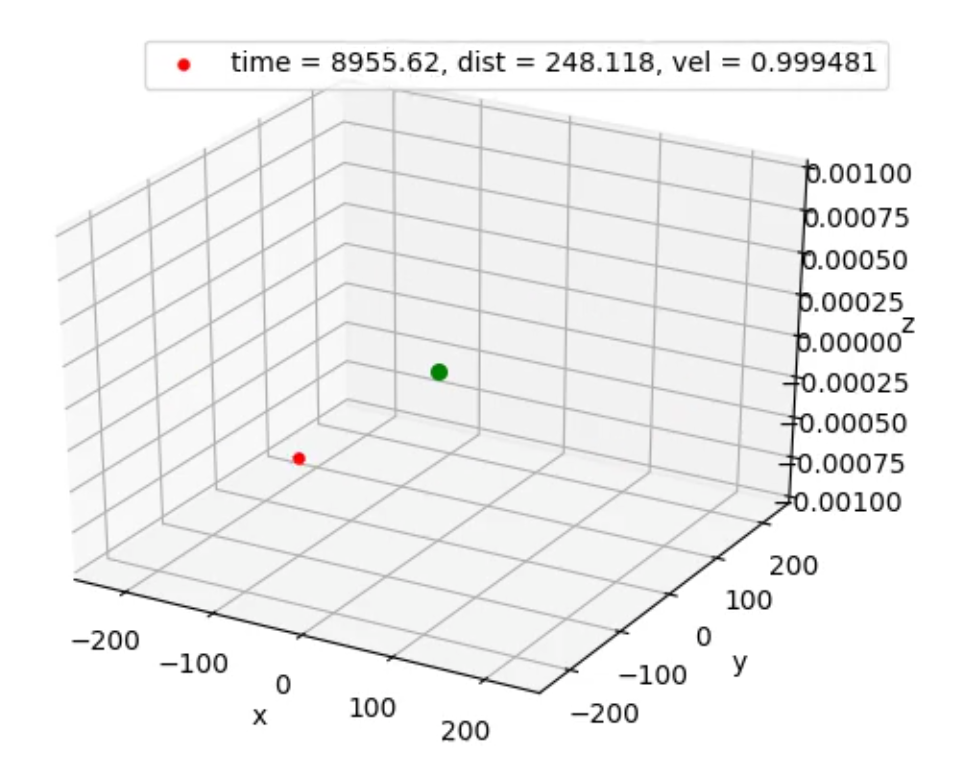
\includegraphics[width=9cm]{cir.png}
	\caption{简单的粒子做圆周运动图片}
	\label{fig:cir}
\end{figure}
\subsection{模型二:匀强磁场中的等距螺旋线运动}
一个简单的磁场模型,即粒子在匀强磁场中做等距螺旋线运动,如图\ref{fig:helix},洛伦兹力不做功,能量守恒。该模型以$0.002s$为步长,模拟约30秒时间内的运动,程序运行用时0.13秒左右。运行中粒子的速度恒为$1.41421m/s$未发生变化,可见模拟精度是比较高的。
\begin{figure}[ht!]
	\centering
	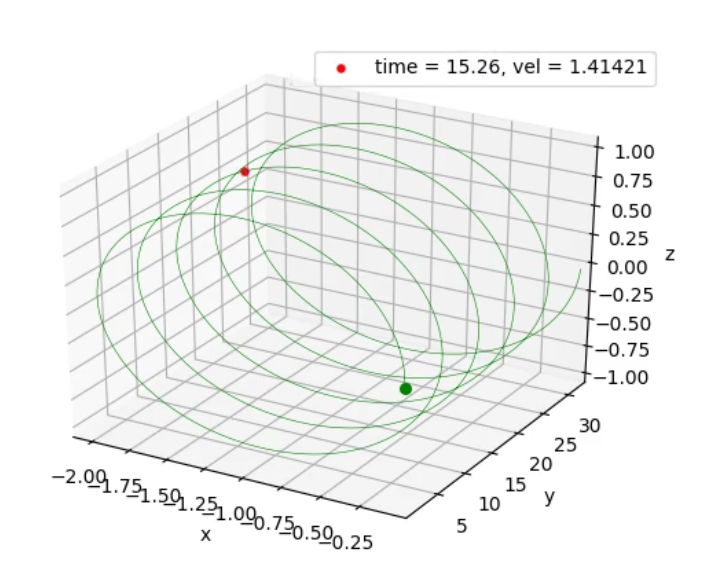
\includegraphics[width=9cm]{helix.png}
	\caption{匀强磁场中等距螺旋线运动图片,运动轨迹已画出}
	\label{fig:helix}
\end{figure}
\subsection{模型三:地磁场束缚带电粒子(磁镜效应)}
地磁场的磁镜效应束缚粒子的模拟,使用两个异号磁荷产生的磁场代表地磁场,如图\ref{fig:globe}。从模拟结果可见,虽然是使用磁荷这个不够严格的模型进行模拟,但由于运动的粒子离磁荷较远,磁荷模型适用较好,结果还是与事实很相符的。如图可见粒子在“地球”(未画出)周围在南北极间来回运动但被约束在离中心一定距离的层中,并朝一个方向“进动”,而小范围内粒子还做螺旋运动,均与事实相符。视频中还可以看到粒子在“赤道”处速度较快且螺旋运动不太明显,而在靠近南北极处震荡剧烈,这是极光的产生原因。粒子速度仅有$10^{-5}$量级的误差。
\begin{figure}[ht!]
	\centering
	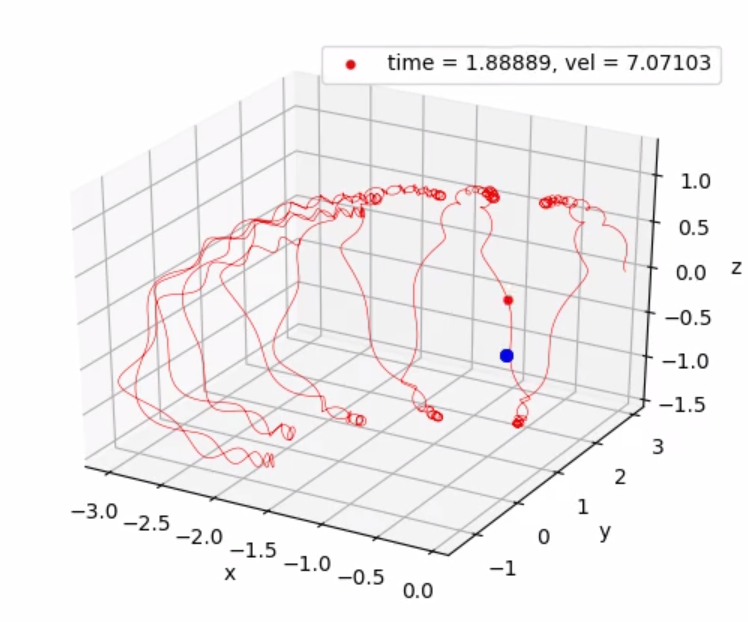
\includegraphics[width=9cm]{globe.png}
	\caption{地磁场中粒子运动的图片,图中大圆点为“地心”,小圆点为运动的粒子,粒子轨迹已画出}
	\label{fig:globe}
\end{figure}
\subsection{模型的代码}
每个模型的模拟需要两个部分的代码,即calc中的具体模型描述和参数设定代码、plot中绘图的描述代码。文中的三个模型calc部分均少于20行代码,plot部分也少于20行代码,并且不同模型绘图代码基本相同,复制后做少量修改即可。


三个模型calc部分代码:
\begin{lstlisting}[language=Python]
    #测试1
    dt = .01
    #trim:仅仅将一部分点写入文件
    trim = 100
    fout.write('%g\n' % (dt * trim))
    timeend = 10 * 2 * math.pi * e ** 2 / (4 * math.pi * epsilon0 * me)
    print('timeend:', timeend)
    q1 = particle(vec(0, 0, 0), vec(0, 0, 0), q=-1 * e, m=0, fixed=1)
    q2 = particle(vec(e ** 2 / (4 * math.pi * epsilon0 * me), 0, 0), vec(0, 1, 0), q=1 * e, m=1 * me, fixed=0)
    h1 = add_particle(q1)
    h2 = add_particle(q2)
    #测试2
    dt = .002
    trim = 25
    fout.write('%g\n' % (dt * trim))
    v = 1
    B = 1e-8
    timeend = 5 * 2 * math.pi * mp / (e * B)
    print(timeend)
    R = mp * v / (e * B)
    print(R)
    def B1(pos, t):
        return vec(0, 1e-8, 0)
    Bconst = field(B1)
    static_B_list.append(Bconst)
    q = particle(vec(0, 0, 0), vec(0, 1, 1), q=e, m=mp, fixed=0)
    add_particle(q)
    #测试3
    dt = .0005
    trim = 1
    timeend = 10
    print(timeend)
    fout.write('%g\n' % (dt * trim))
    k = 100
    def B1(pos, t):
        return mul_num(k * k_m / (dist(pos, vec(0, 0, .001)) ** 3), pos - vec(0, 0, 1)) - mul_num(k * k_m / (dist(pos, vec(0, 0, -1)) ** 3), pos - vec(0, 0, -.001))
    Bconst = field(B1)
    static_B_list.append(Bconst)
    q = particle(vec(0, 3, 0), vec(0, -5, 5), q=+e, m=mp, fixed=0)
    add_particle(q)
\end{lstlisting}
plot部分代码片段,以一个模型为例:
\begin{lstlisting}[language=Python]
ax.scatter(0, 0, 0, color='green', lw=2)
ax.scatter(0, 0, .001, color='blue', lw=2)
ax.scatter(0, 0, -.001, color='blue', lw=2)
xarr = [particle_list_data[i][0].pos.x for i in range(len(particle_list_data))]
yarr = [particle_list_data[i][0].pos.y for i in range(len(particle_list_data))]
zarr = [particle_list_data[i][0].pos.z for i in range(len(particle_list_data))]
ax.plot(xarr, yarr, zarr, color='red', lw=.4)
maindot = ax.scatter(particle_list_data[0][0].pos.x, particle_list_data[0][0].pos.y, particle_list_data[0][0].pos.z, color='blue', lw=.2)
\end{lstlisting}
plot部分每一帧的生成所用函数,即移除旧的点、画出新的点:
\begin{lstlisting}[language=Python]
    global maindot
    maindot.remove()
    maindot = ax.scatter(particle_list_data[ii][0].pos.x, particle_list_data[ii][0].pos.y, particle_list_data[ii][0].pos.z, color='red', lw=.2, \
            label='time = %2g, vel = %2g' % (t * timeend / duration, dist(particle_list_data[ii][0].vel)))
    ax.legend()
\end{lstlisting}
\section{模型的不足之处与可能的改进方案}
\subsection{理论方面的不足}
目前模拟完全不考虑相对论效应以及运动的粒子产生的其他效应,仅仅在经典电磁学方面能够适用,有一定局限性。并且模拟中电磁场可随意给出,不能确定满足高斯定理、环路定理,也有一定缺陷,但可以通过手工检查电磁场函数形式而避免。
\subsection{计算方法的改进}
四阶龙格—库塔法在模拟中表现很好,但考虑到电磁场中运动的性质,如果能使用自适应步长的龙格—库塔法,期望可以有更好的结果。并且目前模型不支持对粒子间相互作用进行龙格—库塔模拟,这是可以改进的一点。而对电流元产生磁场的模拟也不是很理想,因为对于可能出现的粒子离电流元很近时分母接近0的情况目前未能解决。


目前粒子均为点电荷模型,故不能处理可能的粒子碰撞,尤其是正负电荷碰撞的问题,如果能够完善碰撞检测与处理,则能够使得模型的健壮性更强、适用范围更广,成为一个更完善的物理引擎。
\subsection{计算效率的优化}
由于Python作图方便、代码简介,本模拟器使用Python语言实现,但Python运行效率低是众所周知,所以如果使用如C++、Java等语言移植计算部分,将获得进一步运行效率提升。


并且本模拟器以实现功能为重,并未对可能优化的代码部分,如向量计算、迭代计算等部分进行优化,所以提升空间还是很大的。
\subsection{可视化以及用户界面的改进}
本模拟器使用moviepy模块生成视频,目前没有移动视角、缩放等交互式功能,可以考虑使用Unity等高级引擎辅助。


目前模拟器如果想对模型进行模拟,只能通过添加代码、甚至修改代码实现,没有交互式添加粒子、添加电磁场、设定参数的功能,不易于使用,这也是可以改进的一点。
\section{结束}
\textbf{感谢}\\
感谢张增明老师的课程和PPT给此论文很大启发。\\
感谢王泓同学使用龙格—库塔法的建议,以及刘紫檀同学使用pypy提高程序运行速度的建议。\\


\textbf{参考文献}\\
$\left[ 1\right] $张韶华,奚梅成.数值计算方法与算法.北京:科学出版社.2006\\
$\left[ 2\right] $胡友秋等.电磁学与电动力学. 北京:科学出版社.2014
\end{document}









